\documentclass{standalone}
\usepackage{tikz}
\usetikzlibrary{shapes.geometric, arrows.meta}

\tikzset{
    node distance=2cm,
    startstop/.style={rectangle, rounded corners, minimum width=3cm, minimum height=1cm,text centered, draw=black, fill=red!30},
    process/.style={rectangle, minimum width=3cm, minimum height=1cm, text centered, draw=black, fill=orange!30},
    decision/.style={diamond, minimum width=3cm, minimum height=1cm, text centered, draw=black, fill=green!30},
    arrow/.style={thick,->,>=stealth}
}

\begin{document}

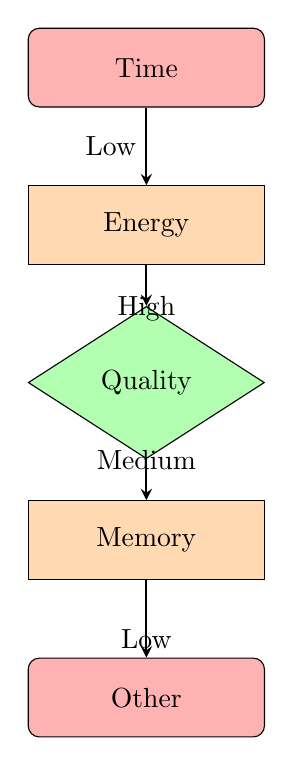
\begin{tikzpicture}[node distance=2cm]

\node (time) [startstop] {Time};
\node (energy) [process, below of=time] {Energy};
\node (quality) [decision, below of=energy] {Quality};
\node (memory) [process, below of=quality] {Memory};
\node (other) [startstop, below of=memory] {Other};

\draw [arrow] (time) -- node[anchor=east] {Low} (energy);
\draw [arrow] (energy) -- node[anchor=north] {High} (quality);
\draw [arrow] (quality) -- node[anchor=south] {Medium} (memory);
\draw [arrow] (memory) -- node[anchor=north] {Low} (other);

\end{tikzpicture}

\end{document}